\subsection{Magnetismus}\label{cap:einlesung_magnetismus}
Magnetische Felder ist für das menschliche Auge nicht sichtbar und trotzdem finden sie ein weites Spektrum an Anwendungsmöglichkeiten in unserer heutigen Gesellschaft. Magnetische Felder dienen zum Beispiel für den Kompass, da die Felder die Nadel immer nach Norden zeigen lässt, oder für Lautsprecher, damit anhand Schwingungen, welche das Magnetische Feld erzeugt, elektrische Signale zu akustischen Signalen umgewandelt werden können.
\newpara
In den folgenden Unterkapiteln wird die Beeinflussung des Magnetfeldes von verschiedenen Metallen und die Erzeugung eines Magnetfeldes durch den elektrischen Strom erklärt.
\subsubsection{Metalle und deren Magnetfeld}
Eisen gilt als ein Metall, welches ein eigenes Magnetfeld erzeugen kann, indem es in Kontakt mit einem Magnet kommt. Ein Metall, welches ein starkes Magnetfeld erhalten kann, wird als magnetisierbar oder in der Physik als ferromagnetisch bezeichnet.
\newpara
Wird ein Eisen-Stück magnetisiert, entstehen zwei Magnetpole: Norden und Süden. Diese Magnetpole dienen nicht zum Herausfinden des Nord- und Südpols, sondern dienen zum Bestimmen der magnetischen Feldlinien (Siehe Abbildung \ref{fig:magnetismus_polarisation_feldlinien}).
\begin{figure}[ht]
  \begin{center}
    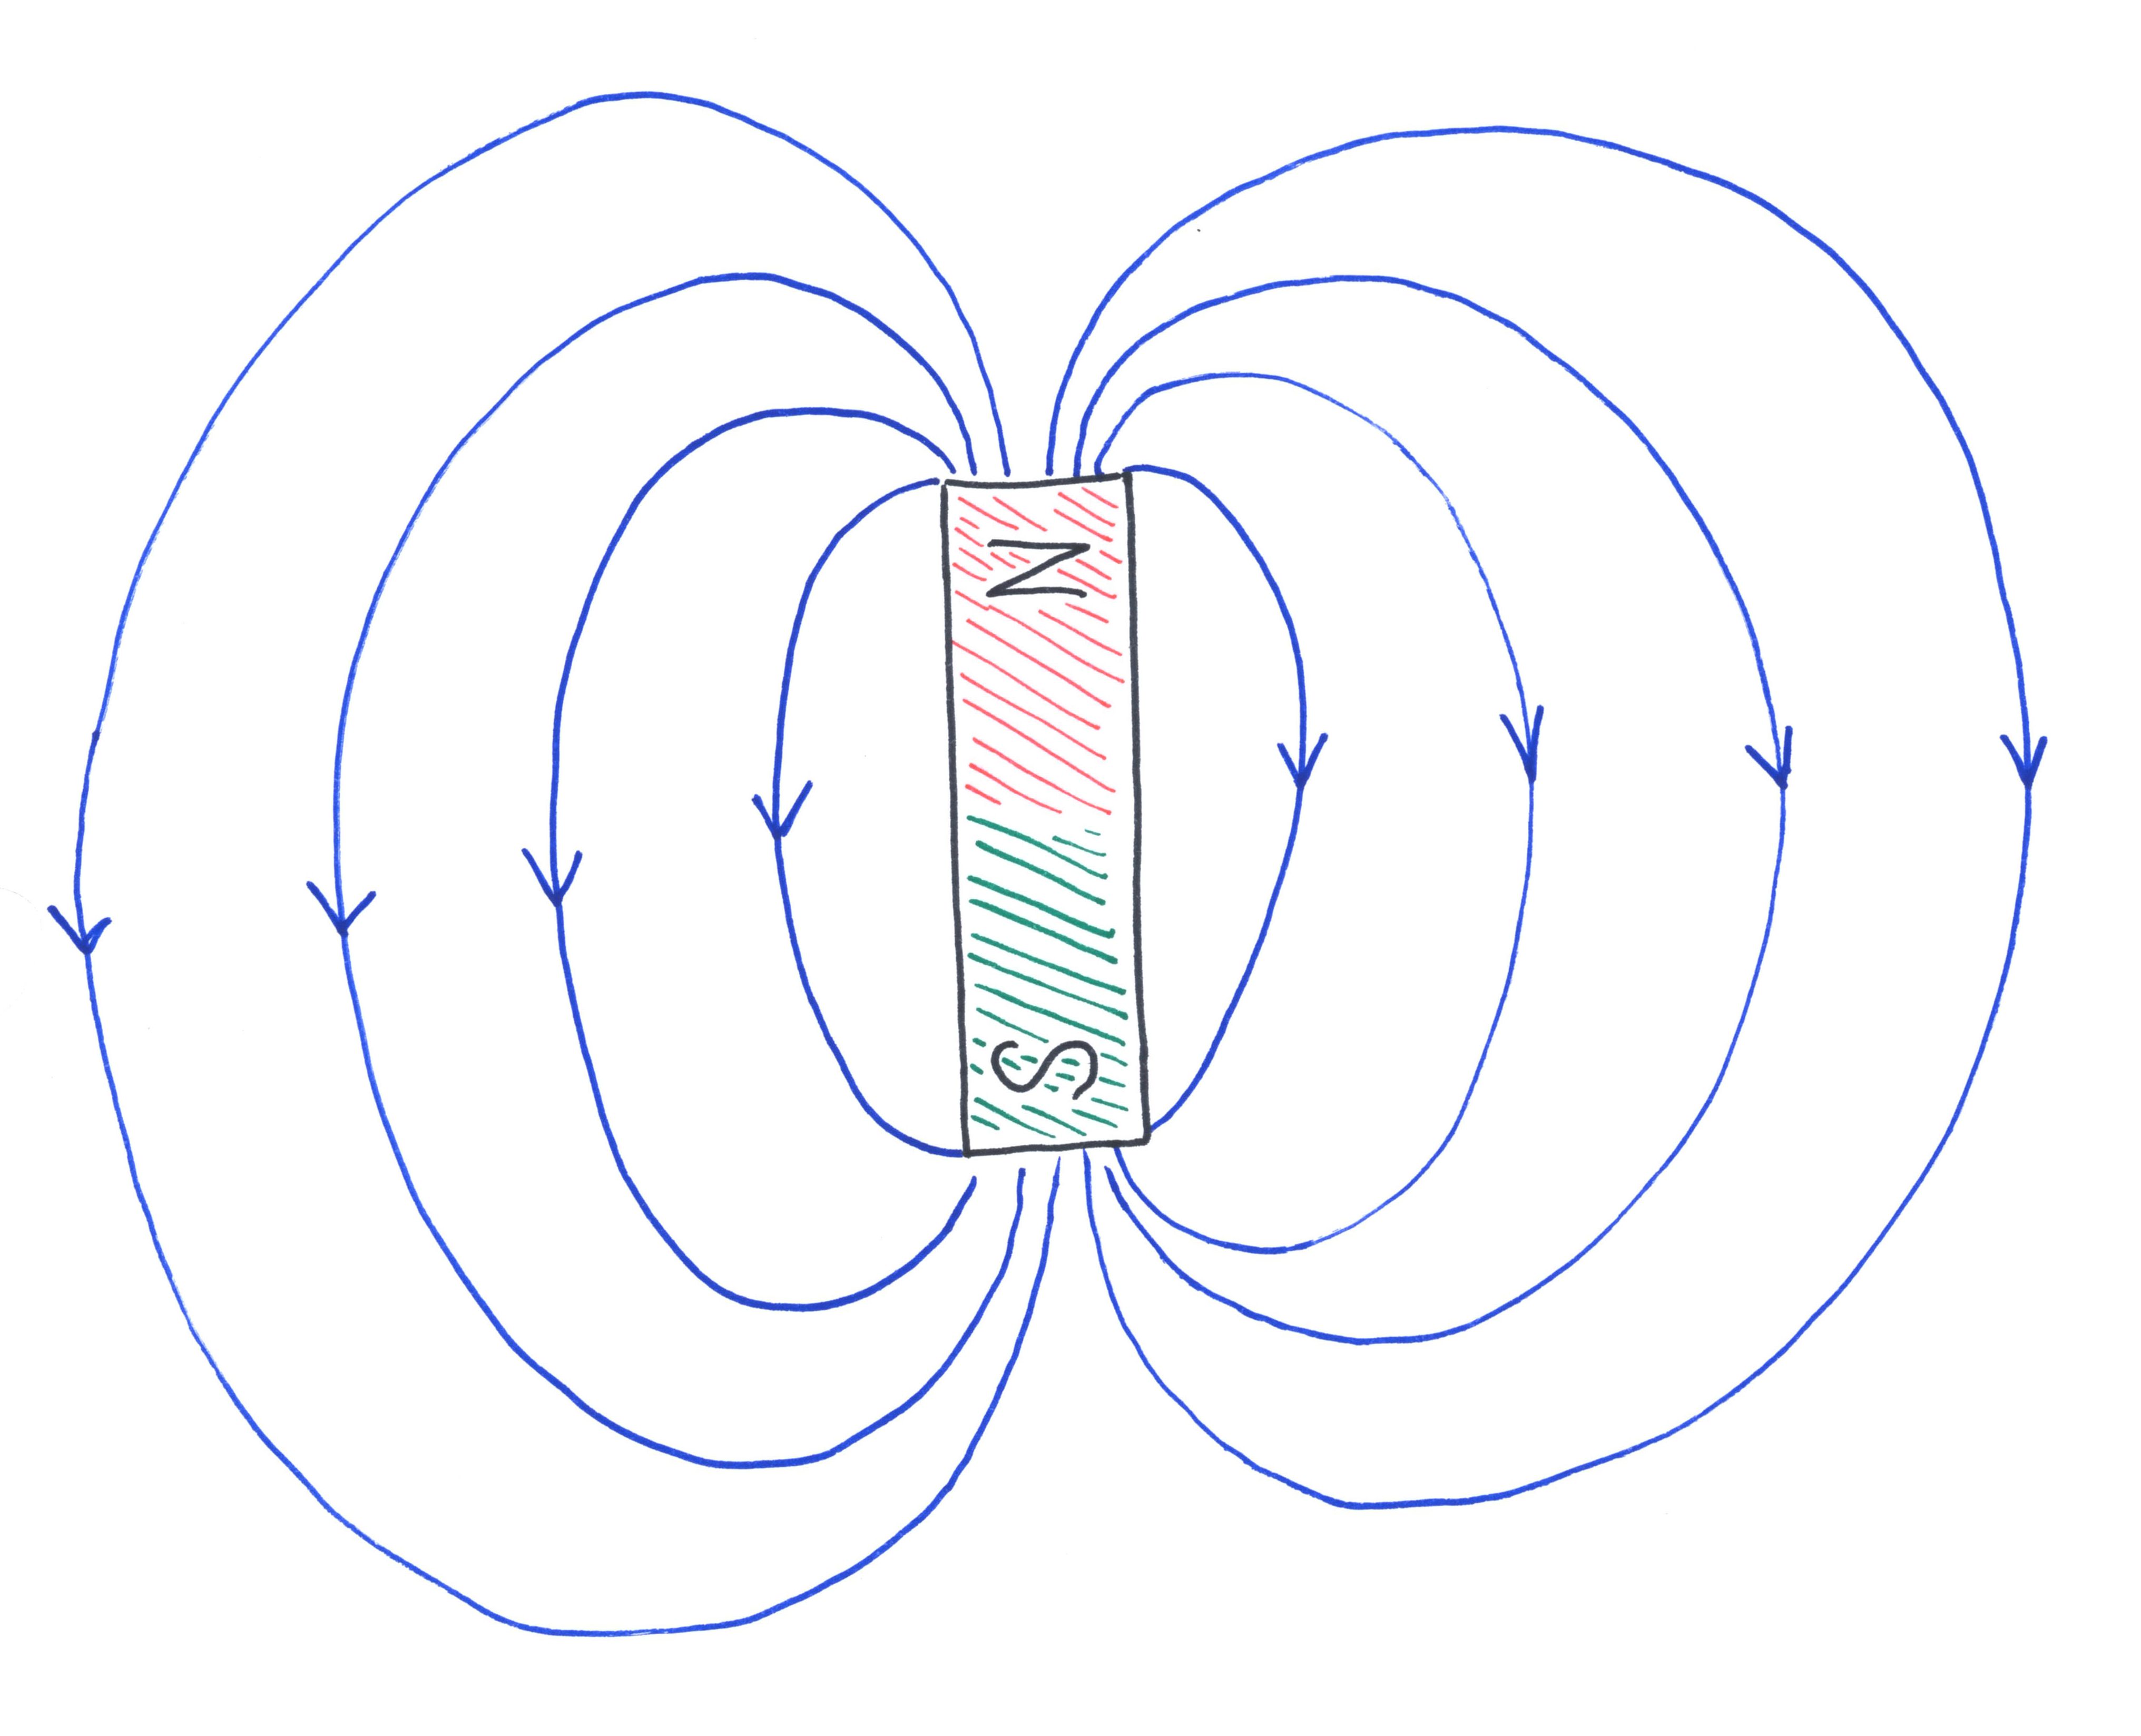
\includegraphics[width=9cm]{assets/images/magnetismus/magnet}
  \end{center}
  \vspace{-3ex}
  \caption{Pole \& Feldlinien eines Magnets}
  \label{fig:magnetismus_polarisation_feldlinien}
\end{figure}

Diese Feldlinien machen wichtige Informationen sichtbar, zum Beispiel wie das Magnetfeld orientiert ist, wie das Magnetfeld von anderen Magnetfeldern beeinflusst wird oder wie stark das Magnetfeld ist (Siehe Abbildung \ref{fig:magnetismus_feldlinien}). Die Stärke wird dabei anhand der Ausbreitung der Feldlinien dargestellt.

\begin{figure}[ht]
    \begin{center}
      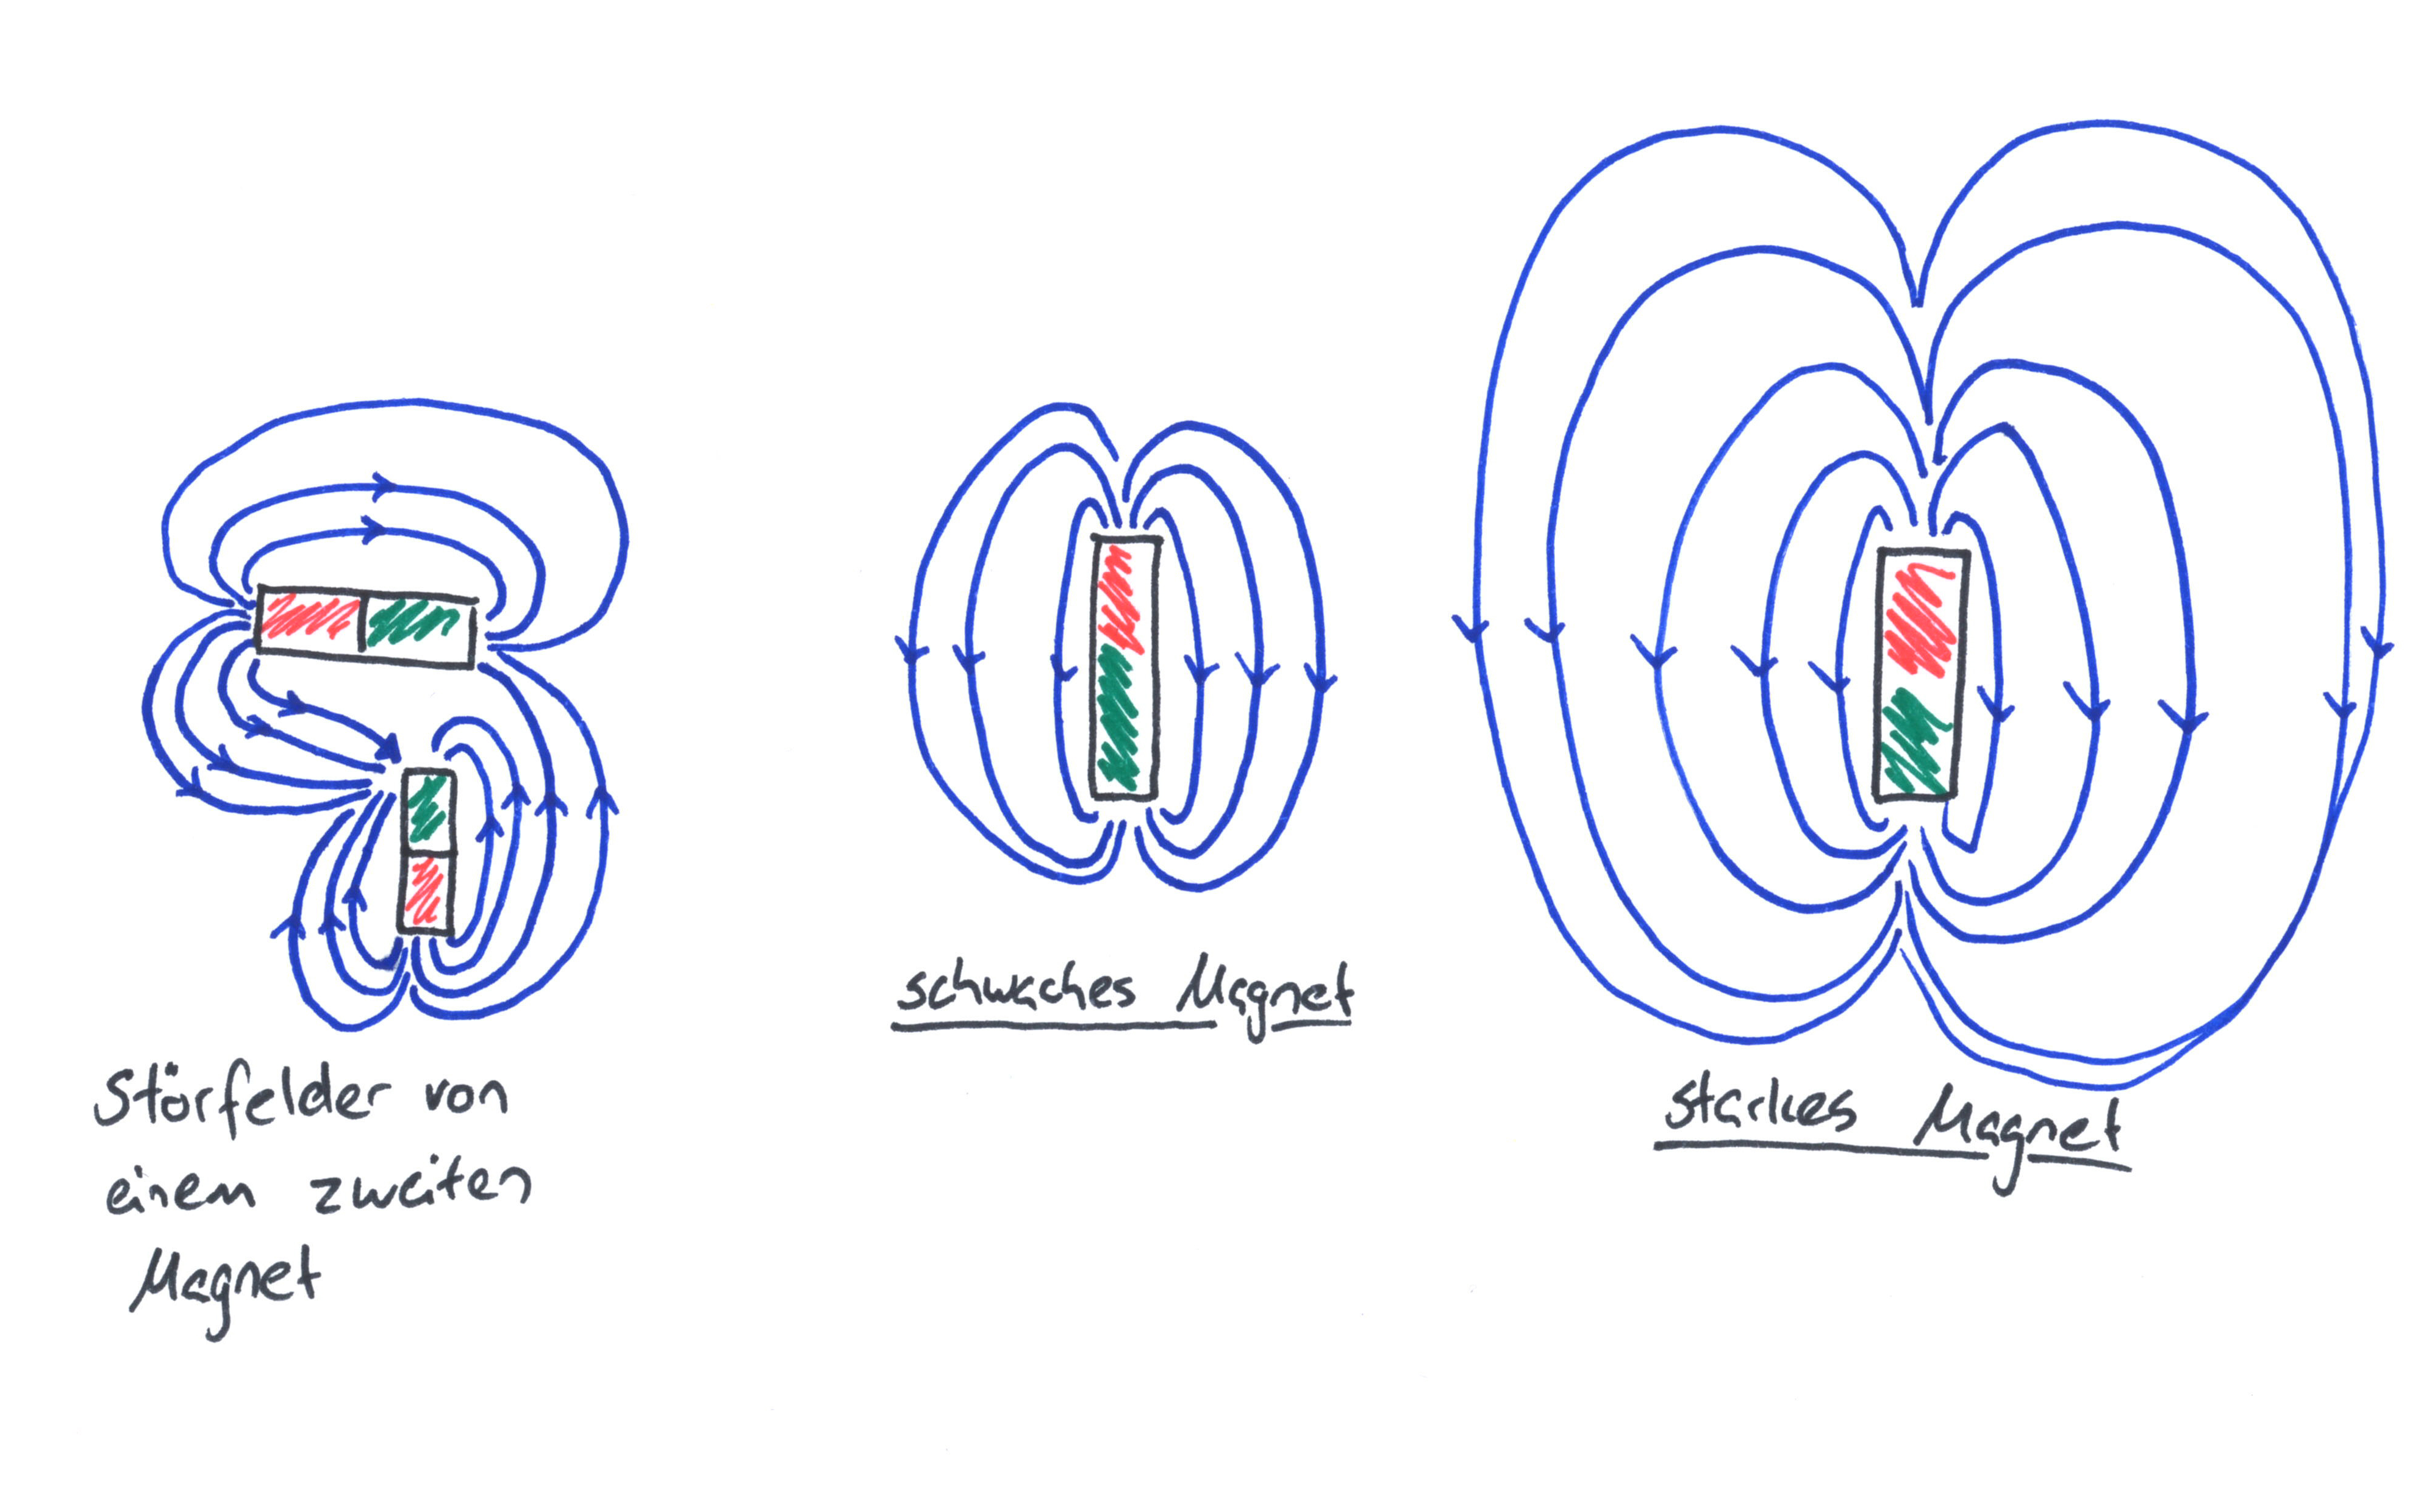
\includegraphics[width=10cm]{assets/images/magnetismus/beeinflussungen_magnet}
    \end{center}
    \vspace{-3ex}
    \caption{Darstellung von Feldlinien}
\label{fig:magnetismus_feldlinien}
\end{figure}

Wie vorher erwähnt, geben Feldlinien an, wie stark ein Magnetfeld sein kann, aber wie kann ein starkes Magnetfeld aufgebaut werden? Das Magnetfeld wird durch die Permeabilität beeinflusst, welche je nach Metall verschieden ist. 
\newpara
Die Permeabilitätszahl kann angeben, ob das Metall magnetisch oder nichtmagnetisch ist. Ein Magnet, welches aus Eisen besteht (Permeabilitätszahl = $300…10’000$) wird nicht dasselbe Magnetfeld eines Aluminium-Magneten (Permeabilitätszahl = $1 + 2.2 \cdot 10^{-5}$) sein, da die Permeabilitätszahl sich untereinander stark unterscheiden. Es kann daher bereits durch Betrachtung der Permeabilität der Metalle herausgefunden werden, ob das Metall magnetisch oder nichtmagnetisch ist. Ein typischer Bereich der Permeabilitätszahl von ferromagnetischen Metallen beträgt $300…10’000$. 
\newpage

\subsubsection{Wirbelstrom}

Der Effekt von Wirbelstrom ist bereits in heutigen grossen Transportmitteln weit verbreitet. Heutige Züge sind, neben normalen Bremsen, mit Wirbelstrombremsen ausgestattet (Siehe Abbildung). Dies ermöglicht den Zügen steile Gefälle befahren zu können, ohne die normalen Bremsen verwenden zu müssen. Lastwagen verwenden ebenfalls Wirbelstrombremsen um bei Gefällen nicht ausser Kontrolle zu geraten (\cite{lokifahrer}).
\begin{figure}[ht]
    \begin{center}
      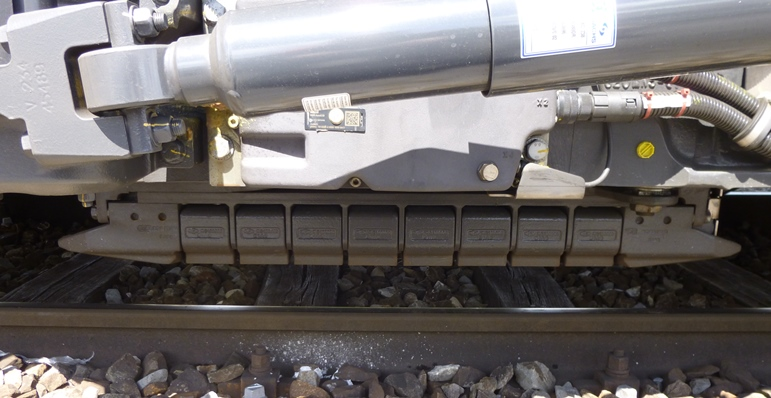
\includegraphics[width=10cm]{assets/images/magnetismus/zug_wirbelstrombremse}
    \end{center}
    \vspace{-3ex}
    \caption{Wirbelstrombremse eines Zuges. Heruntergeladen von \url{http://www.lokifahrer.ch/Lukmanier/Rollmaterial/Bremse/Verschleisslos.htm}}
    \label{fig:zug_wirbelstrombremse}
\end{figure}

Der Wirbelstrom zeigt seinen Effekt nur wenn ein Magnet über eine Platte oder eine drehende Scheibe gezogen wird. Damit nicht zu physikalisch gesprochen wird, wird der Wirbelstrom anhand einem Schlittenbeispiel erklärt. Im folgenden Beispiel wird der Wirbelstrom als die Füsse, welche zum Bremsen verwendet werden, repräsentiert und die Strecke als Elektronenfluss.
\newpara
Man sitzt auf einem Schlitten und fährt eine Strecke herunter. Die Geschwindigkeit des Schlittens erhöht sich konstant, bis es zu schnell wird. Nun drückt man mit den Füssen in den Schnee, um die Geschwindigkeit zu verringern. Man drückt mit der Kraft, welche von den Füssen eingewirkt wird, in den Schnee, was zu einer Reibung und zur Bremsung führt.
\newpara
Wirbelstrom ist also eine Art Energie, welche beim Eindrücken eines Magnetfeldes in eine elektronisch leitfähige Platte erzeugt wird. Der Bremseffekt wird durch \textit{Hineingreifen} des Elektronenflusses erzeugt, was zur Reibung und Bremsung führt (\cite{schulmaterial_magnetismus}). 
\newpage
\subsubsection{Elektromagnetismus}
\say{Elektromagnetismus ist ein Teilgebiet der Physik, das als Elektrodynamik bezeichnet wird.}(\cite{ChemgarooMagnetfelder})
\newpara
Ein Hauptteil der Elektrodynamik beschreibt, dass ein Magnetfeld aufgebaut werden kann, indem elektrischer Strom durch einen Leiter fliesst. Abbildung \ref{fig:rechte_hand_regel} zeigt die Ausrichtung des Magnetfelds bei einem stromdurchflossenem Leiter und eine Darstellung mit der \textit{Rechte-Hand} Regel. Der Daumen zeigt in die Richtung des Stromflusses und die restlichen Finger greifen um den Leiter, was als Magnetfeld bezeichnet wird (\cite{schulmaterial_magnetismus}).

\begin{figure}[ht]
    \begin{center}
      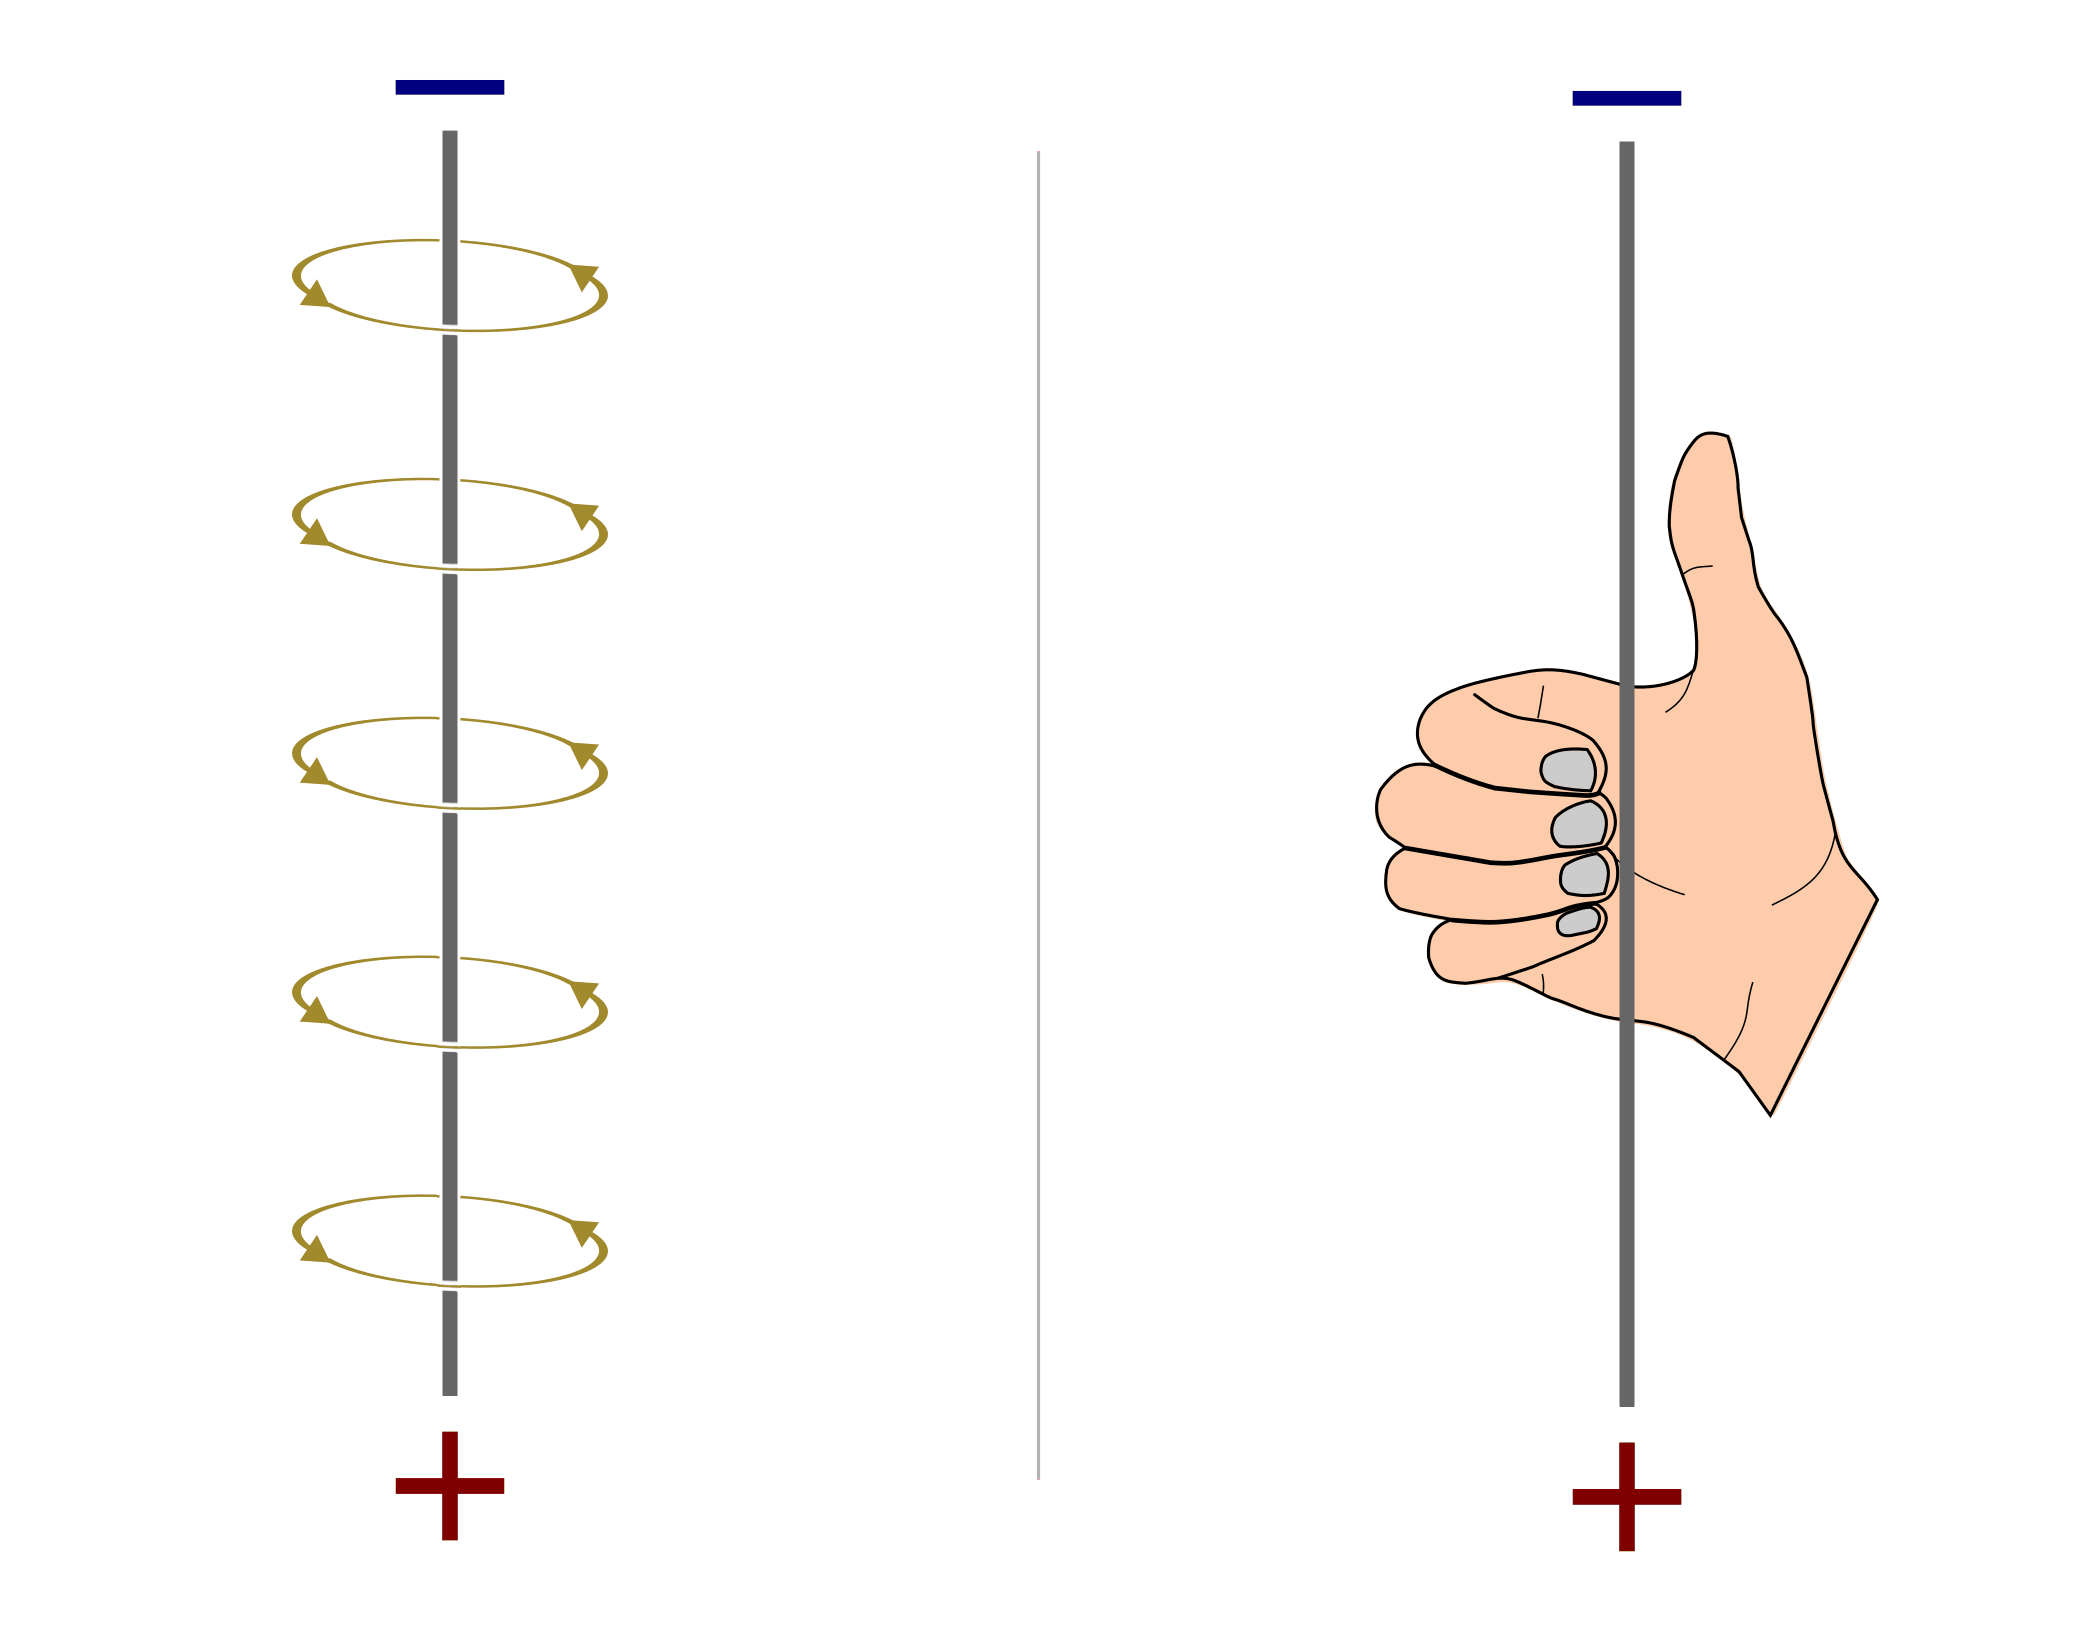
\includegraphics[width=10cm]{assets/images/magnetismus/magnetfeld-leiter-rechte-hand-regel}
    \end{center}
    \vspace{-3ex}
    \caption{Rechte-Hand Regel. Heruntergeladen von \url{https://www.grund-wissen.de/physik/elektrizitaet-und-magnetismus/magnetismus.html}}
    \label{fig:rechte_hand_regel}
\end{figure}

\newpara
Wird ein Kupferkabel, welches um ein Eisenstück gewickelt wurde, mit Strom versorgt, entsteht einen grossen magnetischen Fluss, welcher durch das Eisenstück fliesst (Siehe Abbildung \ref{fig:kupferspule} folgende Seite). Dabei ist zu bemerken, dass sich der Fluss (Abbildung \ref{fig:kupferspule} folgende Seite rechts) jeder Windung zusammensummiert, da alle in die gleiche Richtung fliessen.
\begin{figure}[ht]
    \begin{center}
      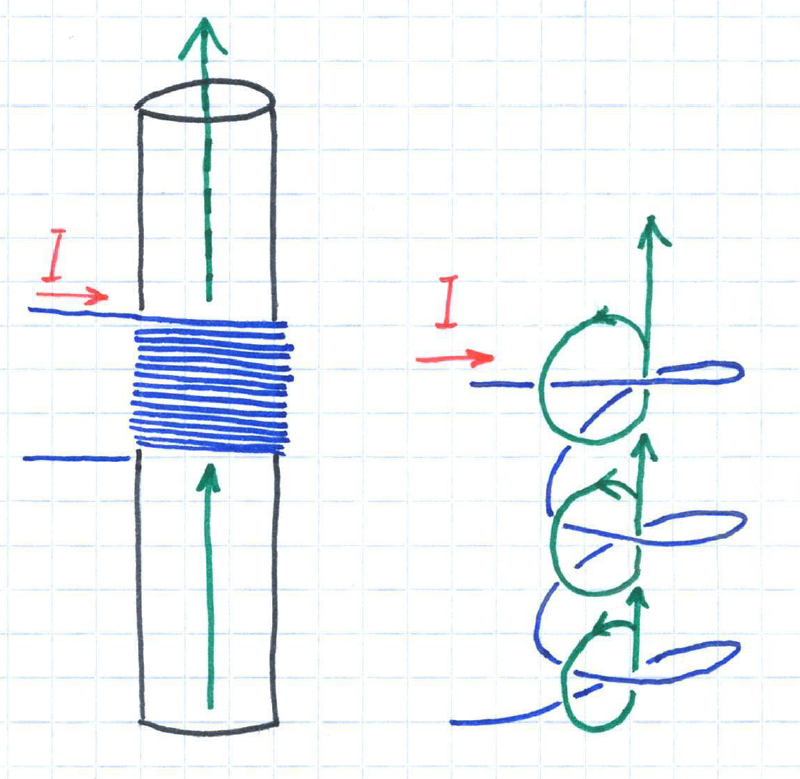
\includegraphics[width=8cm]{assets/images/magnetismus/flussrichtung}
    \end{center}
    \vspace{-3ex}
    \caption{Magnetfluss bei einer Kupferspule}
    \label{fig:kupferspule}
\end{figure}
\newpara
Die Stärke ist bei einem elektrischen Magnet von der Stromstärke und der Anzahl Windungen abhängig (Formel \ref{equ:magnetische_durchflutung_einlesung}). Die Stromstärke dient zur Berechnung der magnetischen Kräfte der einzelnen Windungen. Die Windungszahl wird als Faktor für die magnetischen Kräfte verwendet.
\newpage
\begin{equation}
\label{equ:magnetische_durchflutung_einlesung}
\Theta = N\cdot I
\end{equation}
\begin{gather}
\shortintertext{\textbf{Begriffe:}}
\begin{tabularx}{0.9\textwidth}{ll}
$N$	 &  Anzahl Windungen der Wicklung\\
$I$	 &  elektrische Stromstärke
\end{tabularx}\nonumber
\end{gather}
(\cite[S.452]{kuchling2014taschenbuch})
\begin{comment}
Das magnetische Feld ist die Schlüssel-Komponente der Wirbelstrombremse. Fliesst durch eine, sich drehende Scheibe, ein Magnetfeld, so bewirkt diese eine Elektronenbewegung innerhalb der Scheibe aus. Diese Elektronenbewegung lässt die, in unserem Fall nicht ferromagnetische Scheibe, magnetisch werden. Dies bedeutet, dass sich in der Scheibe nun um das Magnetfeld ein, sich kräftemässig entgegengesetztes Magnetfeld entsteht. Diese Eigenschaft kommt der Wirbelstrombremse zugunsten, welche die Scheibe somit kontinuierlich abbremsen lässt.
\newpara


\begin{figure}[ht]
    \begin{center}
      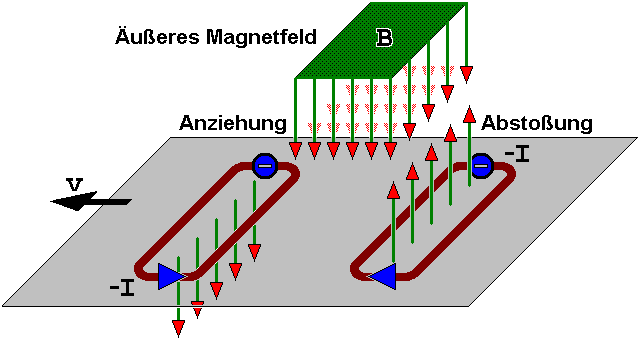
\includegraphics[width=12cm]{assets/images/Eddy_currents_de}
    \end{center}
    \vspace{-3ex}
    \caption[Wirbelstrombremse auf einer Metallplatte]{\centering{Wirbelstrombremse auf einer Metallplatte. Heruntergeladen von \texttt{https://de.wikipedia.org/wiki/Wirbelstrombremse}}}
    \label{fig:eddy_current}
  \end{figure}
\vskip 1cm
Der Wirbelstrom, der sich von der Bewegungsrichtung aus hinter dem Magnet befindet, dreht sich gegen den Uhrzeigersinn. So entsteht ein Magnetfeld in der, sich bewegenden Scheibe, welches mit dem Südpol zum Nordpol schaut. Diese Anziehungskraft wirkt gegen die Bewegung der Scheibe. Der andere Elektronenbewegung, die sich im selben Moment vor dem Magnet befindet, dreht sich allerdings mit dem Uhrzeigersinn. Hier entsteht Ein Magnetfeld, welcher Nordpol sich zum Nordpol des Magneten richtet. Diese Abstossung erzielt ebenso eine Kraft, welche eine Verzögerung auf der Scheibe als Folge hat.
\newpara
Die Scheibe weist eine umso besseren Bremseigenschaft auf, je höher das verwendete Material der Scheibe, den elektrischen Strom leitet. Dies kann damit erklärt werden, da ein Metall, welches einen geringen Widerstand besitzt, viele freie Elektronen mit sich bringt. Somit können auch dementsprechend höhere Wirbelströme entstehen, welche die Scheibe wiederrum bremsen. Die Bremsen erhalten anderseits auch durch Erhöhung des magnetischen Flusses an stärkeren Bremseigenschaften. Durch eine Verringerung des Abstandes, der zwischen Magnet und Scheibe herrscht, kann ebenfalls eine höhere Verzögerung erzielt werden. Die Bremsung erfolgt nicht optimal, wenn der Magnet sich am äussersten Punkt verläuft. Bessere Ergebnisse werden erzielt, wenn sich der Magnet ein wenig tiefer, im Radius befindet. Dies ist indem zu erklären, dass sich andernfalls kein vollständiger Wirbelstrom entstehen kann, welches auch eine schwächere Bremsung als Folge trägt.
\newpara
Prinzipiell ist eine Wirbelstrombremse nicht in der Lage, ein Rad zum Stillstand zu bringen. Um eine Brems-Wirkung zu erzielen, muss bei dieser Wirbelstrombremse eine Elektronenbewegung vorhanden sein, welche kurz vor dem Stillstand noch kaum vorhanden ist. Deshalb bremst dieser, die Scheibe in diesem Punkt so gut wie nicht mehr.
\end{comment}